%   %==========================================================================
%   %  Section
%   %==========================================================================
    \section{アンペールの法則}
%   %==========================================================================
%   %  Subsection
%   %==========================================================================
    \subsection{エルステッドの実験}
        電流が生じている導体のそばに方位磁針をおくと,方位磁針は南北を示さなくなる.
        エルステッド
            \footnote{
                Hans Christian \O rsted ( 1777 - 1851, デンマーク  ):物理学者,科学者.
                太田光一の著した「電磁気学の基礎\I」には,"エールステズ" と片仮名表記されている.
            }
        はこの現象を発見した.その後,更に多くの実験が行われた.そして,アンペールによって,
        \textbf{アンペール力} (2つの電流の間に生じる力) が発見された.アンペール力 $\bF$ は,
        2つの電流を $I$, $I'$ とし,その間の距離を $l$ としたとき,
            \begin{align}
                \bF = k\frac{II'}{l}
            \end{align}
        で表される.$k$ は比例定数である.$k$ の具体的な数値は後で考えることになる
            \footnote{
                SI単位系において,電流の基本単位1[A] はアンペール力と利用し,定義される.
            }.
        2つの電流の間に,引力もしくは斥力(反発力)が発生するということである.
        2つの電流が同じ方向に向いていれば引力が働く.逆向きであれば,斥力が働く.

        原理を考えてみよう.
        電流の周りには磁束密度が生じる.また,電流とは電荷のいどうのことである.
        一方の電流が作る磁束密度の中を,他方の電流のもとである電荷が移動することになる.
        となれば,電荷は磁束密度中をある速度を持って移動することになるので,
        ローレンツ力を受けることになる.電荷というスケールで考えると,
        ローレンツ力を受けているのであるが,電流という大局的な視点で考えれば,
        アンペール力が働いているのである.アンペール力は原理的にはローレンツ力に
        起因するものと考えても良いが,時と場合によって,使い分けることが大事だ.
        例えば,実験や工学的な目的であればアンペール力を利用したほうが便利だし,
        現象を理論的に追求しようとした場合,ローレンツ力として考えたほうが
        一般性が高まることもあるだろう.

        話がそれたが,この節で言いたかったことは,電流の周囲には磁束密度が生じるという
        ことである.では,具体的には,どのような磁束密度が分布しているのだろうか.
        以下で考えていこう.


%   %==========================================================================
%   %  Subsection
%   %==========================================================================
    \subsection{ビオ$=$サバールの法則(復習)}
        \begin{mycomment}
            ビオ$=$サバールの法則についての詳細は,\ref{subsec:BiotSavart_Gene}節を参照.
            以下は,そこからの抜粋である.
        \end{mycomment}
            \begin{myshadebox}{ビオ$=$サバールの法則(電流密度表示)}
                電流はその周囲に磁束密度を発生させる.その発生は以下の
                式に従う.
                \begin{align}
                    \bB(\br)
                    =\frac{\mu_{0}}{4\pi}
                    \int\frac{\bi(\br')\times
                    (\br-\br')
                    }{|\br-\br'|^{3}}\df V'
                \end{align}
            \end{myshadebox}
            \begin{figure}[hbt]
                \begin{center}
                    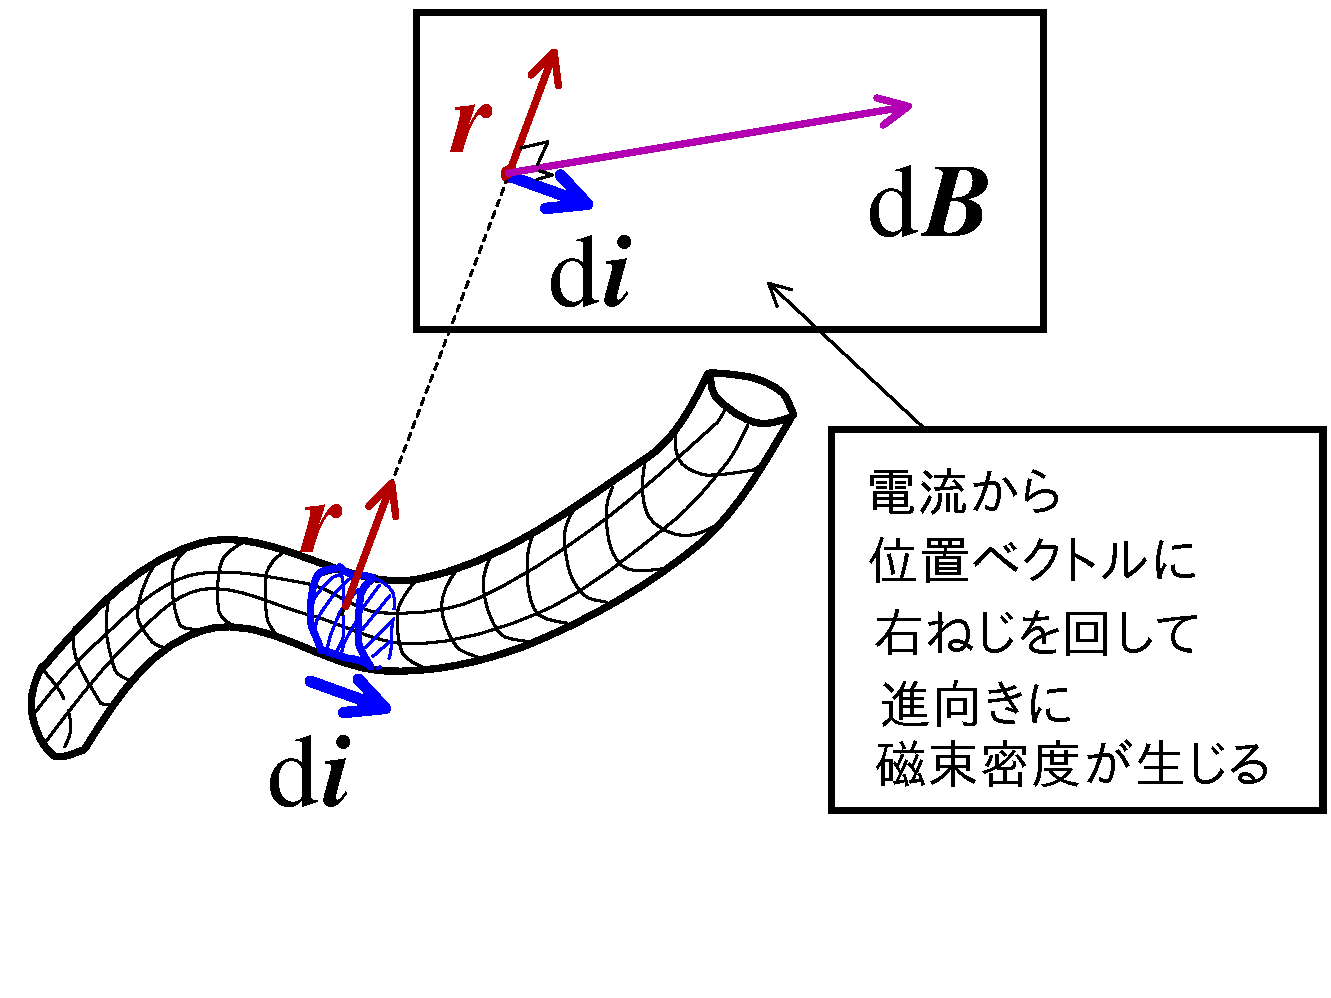
\includegraphics[keepaspectratio, width=7.2cm, height=5.79cm, clip]{biot_savart_1.pdf}
                    \caption{ビオ$=$サバールの法則}
                \end{center}
            \end{figure}

%   %==========================================================================
%   %  Subsection
%   %==========================================================================
    \subsection{アンペールの法則の導出}
%       %======================================================================
%       %  Subsection
%       %======================================================================
        \subsubsection{定常電流}
            ビオ$=$サバールの法則からアンペールの法則を
            導く.はじめに注意しておくと,ビオ$=$サバールの法則は時間変化しない電流
            についての法則である.このような電流を \textbf{定常電流} という.
            従って,以下に導くアンペールの法則も,定常電流を仮定していることになる.
          まず,定常電流を数式で表現しておく.

            電流とは電荷の集団の移動と定義される.電流が時間変化しないということは,
            電荷の移動の時間変化が一定であると考えられる.つまり,電荷密度の
            時間変化はないと解釈できる.ここで,
            電荷保存の法則をおもいだすと,
            \begin{align}
            \frac{\df }{\df t}\int_{\Omega_{S}} \rho(\br,t)\df V
            +\int_{S} \bi(\br,t)\cdot\textit{\textbf{n}}(\br)\df S=0
            \end{align}
            である.電荷密度 $\rho(\br,t)$ が一定の値をとることから,
            この式の第1項は 0 なる.つまり,この式に
            $\frac{\df }{\df t}\int_{\Omega_{S}} \rho(\br,t)\df V=0$ を
            代入して,
            \begin{align}
            \int_{S} \bi(\br,t)\cdot\textit{\textbf{n}}(\br)\df S=0
            \end{align}
            である.この式が定常電流を表現する式である.

%       %======================================================================
%       %  Subsection
%       %======================================================================
        \subsubsection{導出}
            定常電流であることを踏まえてアンペールの法則を導出する.ビオ$=$サバールの法則は
            式(\ref{Bior=savart'slow1})によって,
            \begin{align}
            \bB(\br)
            =\frac{\mu_{0}I}{4\pi}
             \int_{\Gamma}\frac{\bt(\br')\times
             (\br-\br')
            }{|\br-\br'|^{3}}\df s'
            \end{align}
            である.$\bt(\br')\df s'$ とまとめて,
            \begin{align}
            \bB(\br)
            =\frac{\mu_{0}I}{4\pi}
             \int_{\Gamma}\frac{\bt(\br')\df s'\times
             (\br-\br')
            }{|\br-\br'|^{3}}
            \end{align}
            である.
            この式の両辺を曲線 $\Gamma$ を内側に含む閉曲線 $l$ で線積分すると,
            \begin{align}
            &\oint_{l}\bB(\br)\cdot \bt(\br) \df l \notag \\
            &=\frac{\mu_{0}I}{4\pi}\oint_{l}
             \int_{\Gamma}\frac{\bt(\br')\df s'\times
             (\br-\br')
            }{|\br-\br'|^{3}}\cdot \bt^{\ast}(\br)
            \df l
            \end{align}
            とする.ここに,$\bt^{\ast}(\br)\df l$ は 閉曲線 $l$  単位
            接線ベクトル である.この式の右辺に ベクトル解析の公式
            \begin{align*}
            (\bL\times\bM)\cdot\bN
            =(\bN\times\bL)\cdot\bM
            \end{align*}
            を用いると,
            \begin{align}
            &\oint_{l}\bB(\br)\cdot \bt^{\ast}(\br) \df l \notag \\
            &=\frac{\mu_{0}I}{4\pi}\oint_{l}
             \int_{\Gamma}\frac{\bt^{\ast}(\br)\df l\times\bt(\br')\df s'
            }{|\br-\br'|^{3}}\cdot
            (\br-\br')
            \end{align}
            と変形できる.ここで,曲線 $\Gamma$ の単位接線方向ベクトル $\bt(\br')$ と
            閉曲線 $l$ の単位接線成分 $\bt^{\ast}(\br)$ との
            外積 $\bt(\br')\times\bt^{\ast}(\br)$ を
            \begin{align*}
            \textit{\textbf{n}}(\br')=\bt(\br')\times\bt^{\ast}(\br)
            \end{align*}
            とおく.また,$\df S_{l}=\df l\df s'$(「閉曲線 $l$ を縁とする面」という意味)とおく.すると,
            \begin{align}
            \oint_{l}\bB(\br)\cdot \bt^{\ast}(\br)\df l
            =\frac{\mu_{0}I}{4\pi}\oint_{l}
             \int_{S_{l}}\frac{\textit{\textbf{n}}(\br')\df S
            }{|\br-\br'|^{3}}\cdot
            (\br-\br')
            \end{align}
            と書ける.
            さらに曲線 $\Gamma$ が,閉曲線 $l$ の内側にあるので,公式
            \begin{align*}
            &\int_{S_{l}}\frac{\textit{\textbf{n}}(\br')\df S
            }{|\br-\br'|^{3}}\cdot
            (\br-\br') \\
            &=\int_{S_{l}}\frac{\textit{\textbf{n}}(\br')
            }{|\br-\br'|^{3}}\cdot
            (\br-\br')\df S=4\pi
            \end{align*}
            が成り立つ.従って,
            \begin{align}
            \oint_{l}\bB(\br)\cdot \bt^{\ast}(\br)\df l
            =\mu_{0}I
            \end{align}
            となる.この計算では,閉曲線 $l$ の単位接線ベクトルとして,$\bt^{\ast}(\br)$ を
            用いてきたが,ここで改めて,$\bt(\br)=\bt^{\ast}(\br)$ と
            書くことにしても混乱はないので,
            \begin{align}
            \oint_{l}\bB(\br)\cdot \bt(\br)\df l
            =\mu_{0}I
            \end{align}
            さらに,面 $S_{l}$ を流れる電流 を電流密度で表記すると,
            \begin{align}
            I=\int_{S_{l}} \bi(\br)\cdot\textit{\textbf{n}}(\br)\df S_{l}
            \end{align}
            と書けることから
            \footnote{
            この式の $S_{l}$ は閉曲面ではない.$S_{l}$ は
            閉曲線 $l$ を縁とした曲面である. → 電荷保存の法則で考えているのは
            閉曲面 $S$ であって,これとの違いに注意をする.
            },(電流は定常電流である.)
            \begin{align}
            \oint_{l}\bB(\br)\cdot \bt(\br)\df l
            =\mu_{0}\int_{S_{l}} \bi(\br)\cdot\textit{\textbf{n}}(\br)\df S_{l}
            \end{align}
            と表現できる.何度も確認するが,この式の $\bt(\br)$ は
            閉曲線 $l$ の単位接線ベクトルである.
                \begin{myshadebox}{アンペールの法則(積分形)}
                    電流の周囲には磁束密度が生じ,以下の式に従う.
                    \begin{align}
                        \oint_{l} \bB(\br)\cdot\bt(\br)\df l
                        =\mu_{0}\int_{S_{l}} \bi(\br)
                        \cdot\textit{\textbf{n}}(\br)\df S_{l}
                    \end{align}
                \end{myshadebox}

%   %==========================================================================
%   %  Subsection
%   %==========================================================================
    \subsection{法則の意味(図的イメージ)}
        言葉で言えば,「磁束密度 $\bB(\br)$ が
        存在する場所において,任意の閉曲線 $l$ を描き,この閉曲線 $l$ の接線方向に線積分すると,
        その値は閉曲線 $l$ の張る面 $S_{l}$ を貫く電流 $I$ の $\mu_{0}$ 倍に等しい」と言える.
        この式の解釈を簡単にいえば,『電流が磁束密度を生じさせる』ということである.
        つまり,(定常的な)磁束密度が存在するならば,その根源は電流である と言える.

        アンペールの法則を満たす磁束密度は一意に定まらない.そこで,静電場で考えた時と同じように
        磁束密度に対するガウスの法則を導入するのである.このガウスの法則によって,
        磁束密度を一意に決定できるようになる.

%   %==========================================================================
%   %  Section
%   %==========================================================================
    \section{アンペール$=$マクスウェルの法則}
    \begin{mycomment}
        アンペール$=$マクスウェルの法則とは,その記述から察しがつくと
        思うが,アンペールの法則にマクスウェルが改良を加えたものである.
        マクスウェルは,動電磁場を考える場合に,アンペールの法則が不完全
        であるとし,\textbf{変位電流} という新しい概念を導入した.変位電流とは
        なんなのか.マクスウェルはどのように修正したのか.その拡張された
        法則はどういったイメージなのか.この節で考えることにしよう.
    \end{mycomment}

%   %==========================================================================
%   %  Subsection
%   %==========================================================================
    \subsection{アンペールの法則と電荷保存則との矛盾}
        マクスウェルは,アンペールの法則に変位電流の項を加える修正を行った.
        なぜ,このような修正が行われたかというと,アンペールの法則が電荷保存則を
        満たさなかったからである.アンペールの法則は,電荷保存則と矛盾するのだ.
        この矛盾はどういったものなのかを,以下に示す.
            \begin{equation*}
                \drot \bB = \mu_{0}\bi.
            \end{equation*}
        両辺に発散($\ddiv$;divergence)をとってみる.
            \begin{equation*}
                \ddiv( \drot \bB ) = \ddiv ( \mu_{0}\bi ).
            \end{equation*}
        ここで,ベクトル解析の公式から,$\ddiv( \drot \bB ) = 0$ が成立している
            \footnote{
                (公式;定理)任意のベクトル $\bX$ にたいして,
                    \begin{equation*}
                        \ddiv( \drot \bX ) = 0
                    \end{equation*}
                が成立する.
            }.
        つまり,
            \begin{align*}
                \ddiv ( \mu_{0}\bi ) &= 0  \\
                \therefore \quad
                \ddiv \bi &= 0 \,,
                \quad(\because \mu_{0}\mbox{は定数})
            \end{align*}
        となる.ここで,式の見やすさの為に,右辺と左辺を入れ替えた.
        アンペールの法則を認める限り,この式が成立していなければ
        ならないのだけど,一方で,電荷保存則は
            \begin{equation*}
                \ddiv \bi = -\frac{\rd \rho}{\rd t}.
            \end{equation*}
        であり,右辺に関して,$\rd \rho/\rd t \neq 0$ である.
        明らかに,アンペールの法則と電荷保存則は矛盾してしまう.
        どちらが間違っているのだろうか.あるいは,両者とも間違って
        いるのだろうか.マクスウェルの出した答えは,アンペールの法則
        が不完全であるというもので,\textbf{変位電流} という概念を持ち出して,
        修正を加えた.現在では,変位電流の実在性は,電磁波の実験により確固たる
        ものとなっている.

%   %==========================================================================
%   %  Subsection
%   %==========================================================================
    \subsection{変位電流}
        マクスウェルが導入した変位電流とはどのようなものであり,また,
        変位電流の導入はアンペールの法則と電荷保存則の矛盾をどのように解決するか.
        これらを次に確認しよう.
        それには,
        電場に対するガウスの法則に,電荷密度 $\rho$ が現れていることに着目し,
        ここから電荷保存則の式に似せていくという,アプローチをとる.

        電場に対するガウスの法則によれば,
            \begin{align*}
                \ddiv \bE = \frac{1}{\varepsilon_{0}}\rho.
            \end{align*}
        両辺を時間 $t$ で微分する.
            \begin{align*}
                  \frac{\rd}{\rd t}\left(\ddiv \bE \right)
                = \frac{\rd }{\rd t}\left(\frac{1}{\varepsilon_{0}}\rho\right).
            \end{align*}
        ここで,空間に関する微分 $\ddiv$ と時間に関する微分 $\rd/\rd t$ の
        可換性を仮定して
            \footnote{
                時間微分と空間微分は可換であると,信じられている.
                ちなみに,ここに言う「可換」とは,演算の順番のことを言っている.
                つまり,時間微分と空間微分の計算順序を入れ替えてもよい,ということを
                主張している.要は,「空間に関するな微分演算」と「時間」に関する微分演算
                は独立していて,どちらを先に実行しようが,計算結果は変わらないということ.
            },
            \begin{equation*}
                  \ddiv \left(\frac{\rd \bE}{\rd t} \right)
                = \frac{1}{\varepsilon_{0}}\frac{\rd \rho}{\rd t}
            \end{equation*}
        となる.両辺に,$\varepsilon_{0}$ を掛けると,
            \begin{equation*}
                  \ddiv \left(\varepsilon_{0}\frac{\rd \bE}{\rd t} \right)
                = \frac{\rd \rho}{\rd t}.
            \end{equation*}
        最後に,両辺に$-1$をかける.
            \begin{equation*}
                  \ddiv \left( - \varepsilon_{0}\frac{\rd \bE}{\rd t} \right)
                = - \frac{\rd \rho}{\rd t}.
            \end{equation*}
        ここで,再度,電荷保存則の式を見てみよう.
            \begin{equation*}
                \ddiv \bi = -\frac{\rd \rho}{\rd t}.
            \end{equation*}

        電荷保存則と見比べてみると,$- \varepsilon_{0}(\rd \bE/\rd t)$ が
        電流密度と同じ働きをすることが見て取れる.しかし,この項は電流密度そ
        のものを表しているのではない事に注意しよう.
        この項 $\varepsilon_{0}(\rd \bE/\rd t)$ は \textbf{変位電流} とよばれる.

        電場の時間変化 $- \varepsilon_{0}(\rd \bE/\rd t)$ が,電流のように振る舞うように見える.
        考察している範囲に電荷密度が存在していなくとも,電場の時間変化が生じていれば,それを
        電流とみなして良いことを示唆していそうだ.
        アンペールの法則と電荷保存則との矛盾を解く鍵だと言っていい.
        実際にマクスウェルはこの項を持ち出して,アンペールの法則に手を加えて,矛盾を解消した.

%   %==========================================================================
%   %  Subsection
%   %==========================================================================
    \subsection{アンペール$=$マクスウェルの法則の導出}
        アンペール$=$マクスウェルの法則とは,前にも書いた通り,
        アンペールの法則に変位電流の考えを加えたものである.
        その方程式を先に書いてみれば,
        \begin{align}
            \drot \bB
                =   \mu_{0} \bi
                  + \varepsilon_{0} \mu_{0} \frac{\rd \bE}{\rd t}.
        \end{align}
        この方程式は,アンペールにより発見された \textbf{アンペールの法則} に,
        マクスウェルが修正を加えたもので,\textbf{アンペール$=$マクスウェルの法則} と
        よばれる.

        式の形を見るとは,単に,アンペールの法則の右辺に,
        変位電流を加えただけだ.しかし,電荷保存則との矛盾が解消されている.
        右辺第二項の $\varepsilon_{0} \mu_{0} (\rd \bE/\rd t)$ が
        あるため,$\ddiv \bi=0$ となっても,
                \begin{equation*}
            \drot \bB = \varepsilon_{0} \mu_{0} \frac{\rd \bE}{\rd t}.
                \end{equation*}
        となって,電荷保存則と矛盾はしない.
        この式を解釈すると,電場の時間変化が回転する磁場を発生させる,
        ということになる.

%   %==========================================================================
%   %  Subsection
%   %==========================================================================
    \subsection{法則の意味(図的イメージ)}

%   %==========================================================================
%   %  Section
%   %==========================================================================
    \section{静電容量}
%   %==========================================================================
%   %  Subsection
%   %==========================================================================
    \subsection{キャパシタンス}

    \begin{memo}{「キャパシタ」と「キャパシタンス」の違い}
    \end{memo}

%   %==========================================================================
%   %  Subsection
%   %==========================================================================
    \subsection{変位電流とキャパシタ}

%   %==========================================================================
%   %  Subsection
%   %==========================================================================
    \subsection{平行平板型のキャパシタ}

%   %==========================================================================
%   %  Section
%   %==========================================================================
    \section{電流のSI単位に基づく定義}
%   %==========================================================================
%   %  Subsection
%   %==========================================================================
    \subsection{直線電流が作る磁束密度}
        さて,今まで電流の単位として [A]=[C・s] を用いてきたが,
        先にも書いたように,これは現実の定義とは違うものである.
        SI単位系における基本単位は,電荷ではなく,電流が
        採用されている.

        今までの議論で電流を定義するための準備
        ができたので,そのための準備としてのこの項目と,次も項目で,
        電流の定義をし直すことにする.

        まず,定義の概略を示しておく.電流は電荷の移動によって生じる現象であるので,
        電流はローレンツ力を受ける.この電流に対するローレンツ力を人間が観測する
        するときは,導線が受ける力として観測される.
        その力は $\bF=\textit{\textbf{I}}\times \bB$ で表現できた.
        ここで,2つの平行な直線の導線を用意する.この2つの導線に同じ向きに電流を流すと,後に示すように,
        導線が互いに引き合う現象が生じる
        \footnote{
            電流を逆向きに流せば,導線同士は互いに反発しあう.
        }
        .この力によって電流を定義するのである.実際の力の大きさとしては $2\times 10^{-7}$ [N/m] が
        採用されている.
        導線同士が互いに引き合うのはローレンツ力によるものであり,これは
        一方の電流の作る磁束密度が,他方の電流(電荷)に及ぼすローレンツ力である.
        従って,1つの導線に流れる電流が作る磁束密度を計算する必要があり,
        ここではその計算をすることが目的である.そして,次の項目でここでの計算結果を
        利用して,電流を定義していこうと考える.

        直線電流が図\ref{fig:den_jisoku}のような磁束密度を作ることを確認する.
        1本の直線な導線を用意する.この導線に定常電流 $\textit{\textit{i}}$ を流し,
        この定常電流がその周囲に作る磁束密度を考える.
        アンペールの法則は
                    \begin{align}
                        \oint_{l} \bB(\br)\cdot\bt(\br)\df l
                        =\mu_{0}\int_{S_{l}} \bi(\br)
                        \cdot\textit{\textbf{n}}(\br)\df S_{l}
                    \end{align}
        のように書かれる.
            \begin{figure}[hbt]
                \begin{tabular}{cc}
                    \begin{minipage}{0.5\hsize}
                \begin{center}
                    \includegraphicsdouble{den_jisoku.pdf}
                    \caption{電流の作る磁束密度}
                    \label{fig:den_jisoku}
                \end{center}
                    \end{minipage}
                    \begin{minipage}{0.5\hsize}
                \begin{center}
                    \includegraphicsdouble{den_lorentz.pdf}
                    \caption{電荷の磁束密度から受けるローレンツ力}
                    \label{fig:den_lorentz}
                \end{center}
                    \end{minipage}
                \end{tabular}
            \end{figure}

        磁束密度の大きさは,ビオ$=$サバールの法則から,
        導線から等距離にある部分では等しくならないといけない.
        従って,直線の導線の任意の点を流れる電流が起こす,磁束密度の
        大きさが等しい部分をつないでいけば,その形は閉じた
        円になる.そして磁束密度の向きは電流の生じる方向に対して
        右回りである.図\ref{fig:den_lorentz}参照.これがわかれば,
        アンペールの法則の左辺;$\oint_{l} \bB(\br)\cdot\bt(\br)\df l$ の
        積分経路は,円にとればよいことがわかる.

        積分経路を円とすれば,その半径を $r$ とした場合に,
        磁束密度の強さは,以下のように計算される.

        アンペールの法則の左辺を計算すると,
            \begin{align*}
                \mbox{(左辺)}=\oint_{l} \bB(\br)\cdot\bt(\br)\df l
                      =\oint_{l}B\,\df l=B\oint_{l}\,\df l
            \end{align*}
        ここで,積分経路 $l$ は円であるので,$\oint_{l}\,\df l=2\pi r$ である.従って,
            \begin{align*}
                \mbox{(左辺)}=2\pi rB
            \end{align*}
        右辺;$\mu_{0}\int_{S_{l}} \bi(\br)\cdot\textit{\textbf{n}}(\br)\df S_{l}$ は,
        定常電流であるので,これは $\mu_{0}I$ と書ける.

        以上から
            \begin{align*}
                2\pi rB=\mu_{0}I
            \end{align*}
        すなわち,
            \begin{align}
                B=\frac{\mu_{0}I}{2\pi r}
            \end{align}
        である.

        \begin{memo}{積分経路を円にとる}
            なぜなら,円でない曲線経路を
            とったとしても,磁束密度の向きは円方向を向いているからである.
            下図参照.
                \begin{figure}[hbt]
                    \begin{center}
                        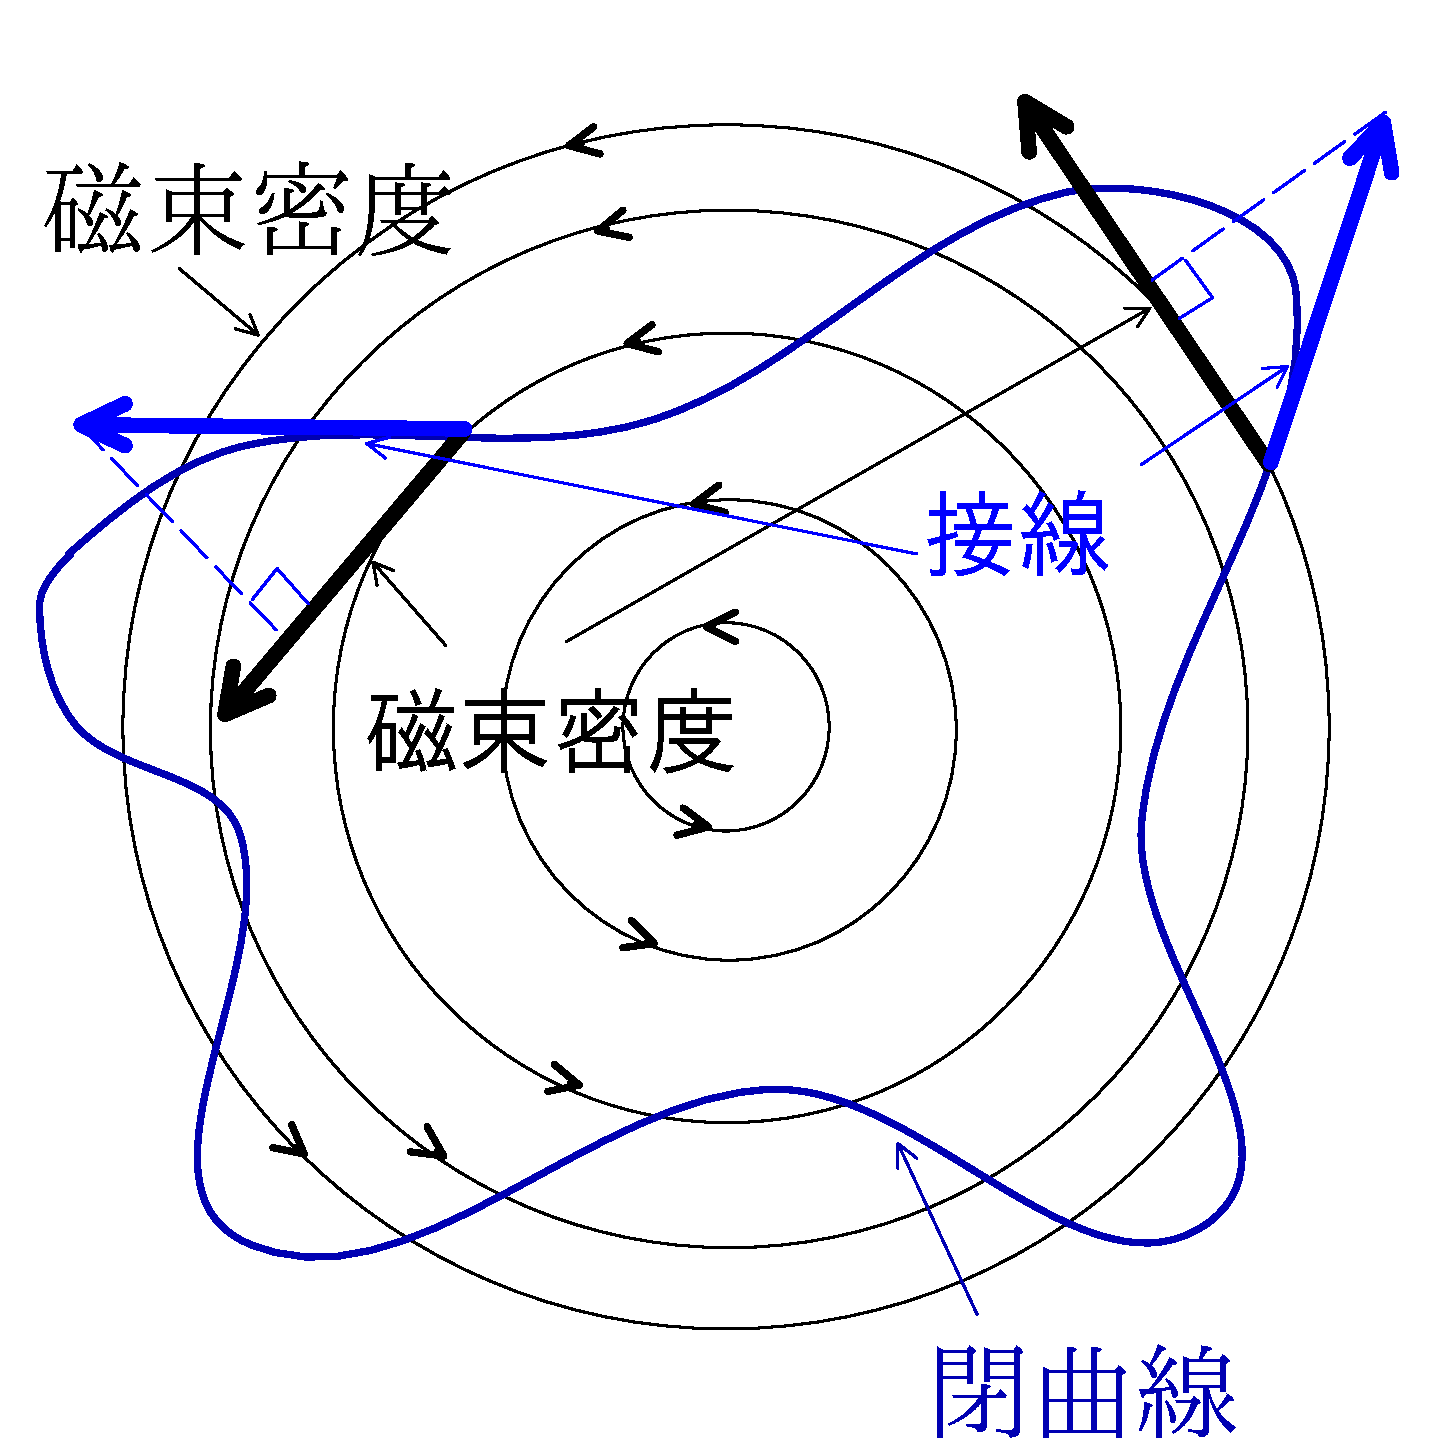
\includegraphics[keepaspectratio, width=6cm,height=6cm,clip]{dentei1.pdf}
                        \caption{閉曲線の取り方}
                        \label{fig:dentei1}
                    \end{center}
                \end{figure}

            図で示したように,曲線の接線と磁束密度の内積をとるので,
            接線の磁束密度に直角な方向成分は考察する必要がないのである.
            (考えたとしても,内積は0となるので意味がない.)
        \end{memo}

%   %==========================================================================
%   %  Subsection
%   %==========================================================================
    \subsection{電流が受ける力}
            電気量 $q$,速度 $\bv$  をもつ1つの電荷が受けるローレンツ力 $\bF$ をおもいだすと,
            \begin{align}
            \bF=q\bv\times\bB
            \end{align}
            であった.
            複数の電荷を考えれば,電荷密度という概念を導入して,
            \begin{align}
            \bF=\left(\int_\Omega \rho(\br)\df V\right)
            \langle\dot{\br}\rangle\times\bB
            \end{align}
            ここに,$\langle\dot{\br}\rangle$ は電荷のドリフト速度である.
            ドリフト速度というのは,複数の電荷の移動速度の平均である.
            そして,$Q:=\int_\Omega \rho(\br)\df V$ おくと,
            $\bF=Q
            \langle\dot{\br}\rangle\times\bB$ と書けて,
            $Q\langle\dot{\br}\rangle$ は電流を表現していると考えられるから,
            これを $\textit{\textbf{I}}$ おくことで($\textit{\textbf{I}}:= Q\langle\dot{\br}\rangle$),
            \begin{align}
            \bF=\textit{\textbf{I}}\times\bB
            \end{align}
            を得る.

%   %==========================================================================
%   %  Subsection
%   %==========================================================================
    \subsection{電流の定義(1[A]の定義)}\label{denryuuteigi}
            電磁気学ではSI単位系において,電流の単位が基本単位として
            採用されている.ここではその基本単位となる電流の1[A]を
            定義する.一つ前の項目\ref{dennryuunoukerutikara}で
            電流が受ける力は,導線の受ける力として現れることを確認し,
            その力は式(\ref{denruu_F})で表された.それをもう一度
            書き下せば,
                \begin{align}
                    \bF=\textit{\textbf{I}}\times \bB
                \end{align}
            である.
            \begin{figure}[hbt]
                    \begin{center}
                        \includegraphicsdefault{denryu_teigi.pdf}
                        \caption{電流の定義の説明図1}
                        \label{fig:denryu_teigi}
                    \end{center}
                \end{figure}

            2本の平行に並んだ導線を用意する.導線の名前をそれぞれ1,2とする.
            この2本の導線に定常電流を流す.それら2つの定常電流を
            それぞれ $\textit{\textit{i}}_{A}$,$\textit{\textit{i}}_{B}$ と
            する.この内の一方の導線に流れる電流が作る磁束密度を考える.
            どちらでもよいが $\textit{\textit{i}}_{1}$ の作る磁束密度を考える.
            アンペールの法則より,
                \begin{align*}
                    \oint_{l} \bB(\br)\cdot\bt(\br)\df l
                    =\mu_{0}\int_{S_{l}} \bi_{1}(\br)
                    \cdot\textit{\textbf{n}}(\br)\df S_{l}
                \end{align*}
            これは前項目で計算計算したように,
                \begin{align*}
                    B=\frac{\mu_{0}I_{1}}{2\pi r}
                \end{align*}
            である.従って,他方の導線に与える力は,
            (電流と磁束密度のなす角は $\pi/2$ であることに注意して)
                \begin{align*}
                    F=I_{2}B\sin\frac{\pi}{2}=I_{2}B
                \end{align*}
            従って,$B=\mu_{0}I_{1}/2\pi r$ を代入すれば.
                \begin{align}
                F=\frac{\mu_{0}I_{1}I_{2}}{2\pi r}
                \end{align}
            である.
            この式を用いて1[A]の電流を定義する.図\ref{fig:AARA}に描いたように,
            重さ $2\times10^{-7}$[N] のおもりを,同線の片方につるす.
                \begin{figure}[hbt]
                    \begin{center}
                        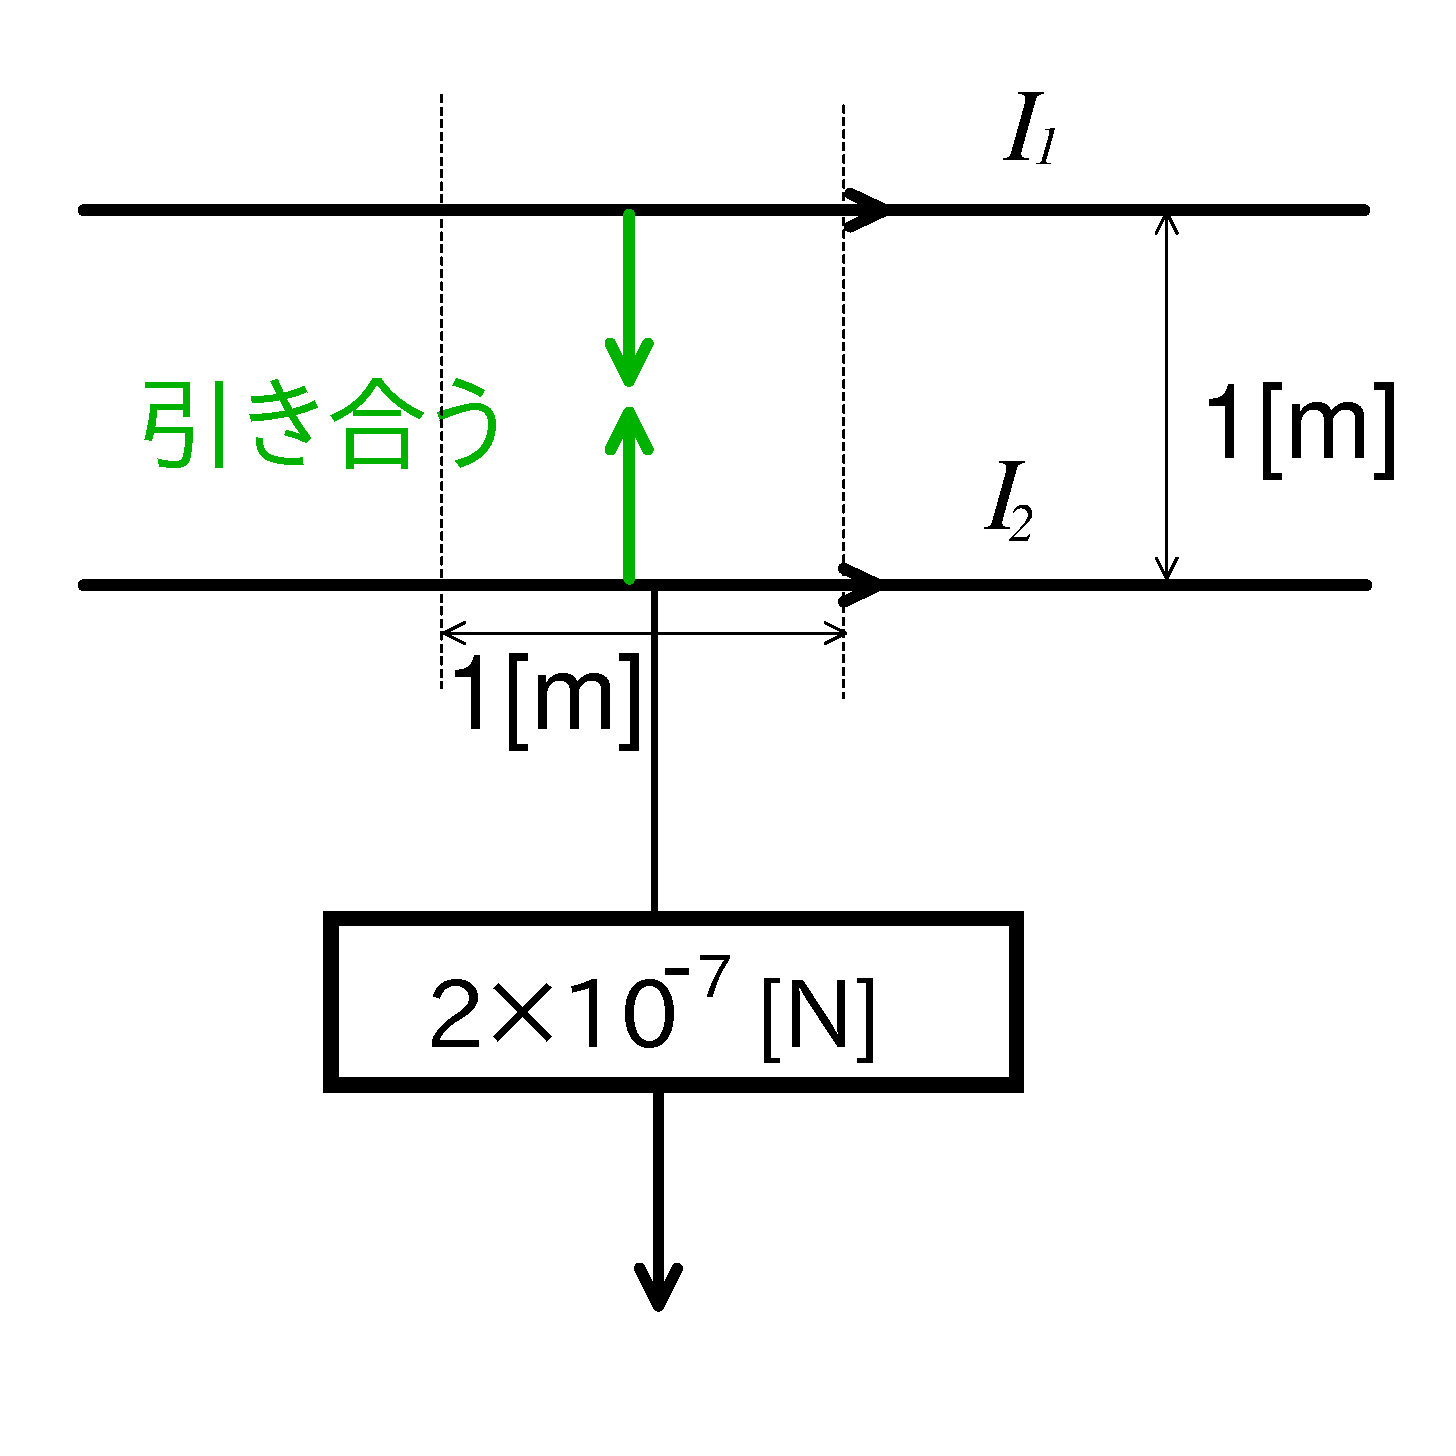
\includegraphics[keepaspectratio, width=5cm,height=4.5cm,clip]{AARA.pdf}
                        \caption{電流の定義の説明図2}
                        \label{fig:AARA}
                    \end{center}
                \end{figure}

            このとき,各導線には同じ方向に電流が流れているとする.
            導線間の距離は1[m]としている.
            この状態で,釣り合いが取れたとき,1[A]の電流が流れていると
            定義するのである.

            以上のことを形式的にまとめておこう.
                \begin{myshadebox}{電流1[A]の定義}
                    1[m]の間隔をおいた
                    2本の平行導線に電流を流して,
                    この導線に働く力が単位長さ(1[m])当たり $2\times10^{-7}$[N] の
                    力が働くとき,
                    この時に流れる電流を1[A]
                    と定義する.
                \end{myshadebox}
